\chapter{任务一:声学参数}
\label{chap:task1}

\section{显示和查看 SoundEditor 中的功能}

打开 Praat, 在 Object window 中点击 Open $rightarrow$ Read from file..., 导入 GuoL/40004.wav 文件。
然后选中该项目,点击 View \& Edit, 进入 SoundEditor window。
进去之后默认只展示波形waveform、语谱图spectrogram和部分其他信息。

我们可以在菜单栏依次选中 Show Pitch/Intensity/Formant/Pulses来展示音强intensity、基音轮廓pitch contour、共振峰formant和脉冲pulses。

\begin{figure}[H]
  \centering
  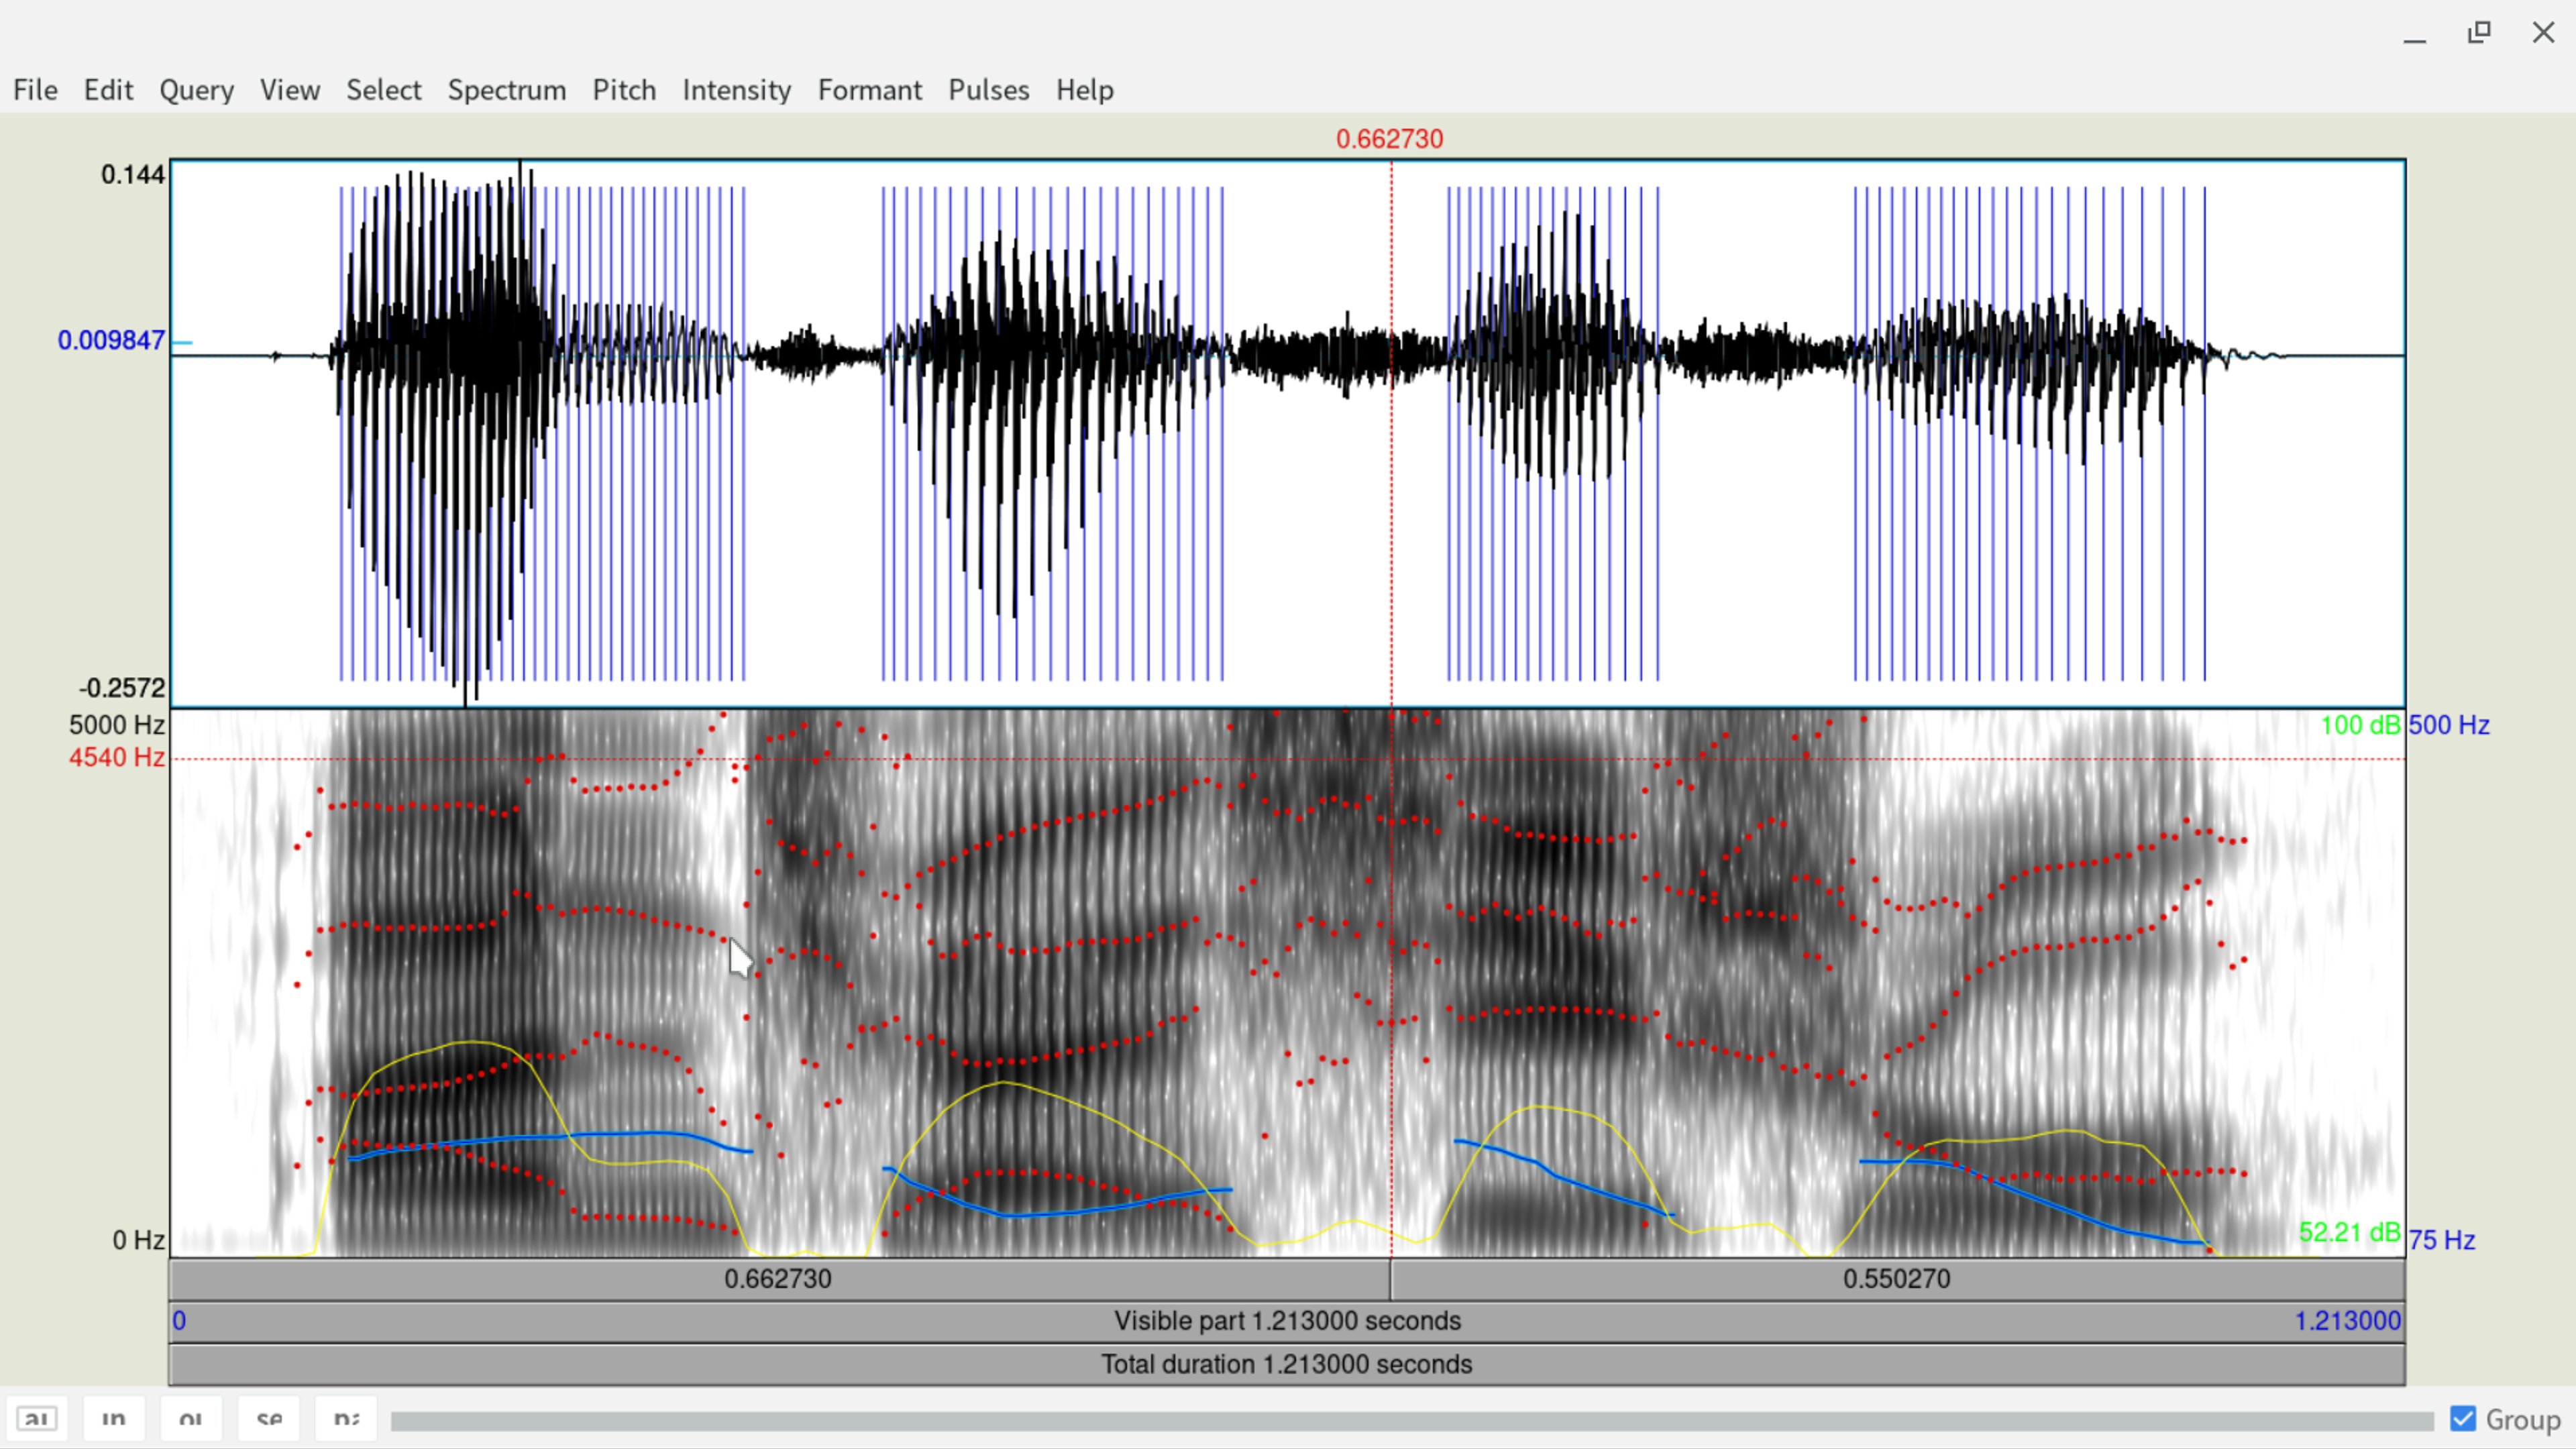
\includegraphics[width=16cm]{praat_sound_editor.png}
  \caption{Praat SoundEditor 界面概览}
  \label{fig:praat_sound_editor}
\end{figure}

图~\ref{fig:praat_sound_editor} 展示了一个典型的 SoundEditor 界面,该界面的图形与对应的项目有:

\begin{enumerate}
  \item \textbf{波形waveform}: 界面上半部分中黑色的内容就是波形图,可以在右下角对波形图进行缩小放大以及移动查看范围。横轴为时间,纵轴为音强。左侧上下两个黑色数字展示的数值区间。
  \item \textbf{语谱图spectrogram}: 语谱图(频谱图)为界面下半部分的黑色内容。横轴跟波形图一样是时间,纵轴是频率。左侧上下两个数字展示的显示的频率区间的上下界(单位:Hz),一般下界是 0 Hz, 上界是 5000 Hz。语谱图中黑色内容的灰度代表对应频率的能量密度(振幅)大小,颜色越深代表能量越大。
  \item \textbf{音强intensity}: 下半部分中黄色曲线就代表音强,右侧绿色字体就是刻度,单位为 dB。
  \item \textbf{基音轮廓pitch contour}: 下半部分中蓝色的点(线条)表示基音频率 $F_0$,右侧蓝色字体表示刻度,对于清音(白噪声)是没有基音频率的。男性的 $F_0$ 一般在 $[80, 200]$ 之间,而女性和儿童在 $[150, 250]$ 和 $[200, 500]$。不过有研究表明不同声带的人之间 $F_0$ 范围变化比性别之间的差距更大。
  \item \textbf{共振峰formant}: 下半部分红色的点(线条)表示共振峰,默认显示五个共振峰:$F_1, F_2, F_3, F_4, F_5$。
  \item \textbf{脉冲pulses}: 上半部分的蓝色竖线就是(声门)脉冲。
\end{enumerate}

\section{比较和解释不同设置参数}
\subsection{语谱图}
在语谱图的设置中,我们可以设置查看频率范围(View of range),这可以改变语谱图频率的显示范围和密度。窗口长度(Window length)用于指定傅立叶变换的时间窗口大小,长度越大的窗口的频率分辨率(不同频带的区分度)会越大,不过其时间分辨率就会减小

Dynamic range 长度用于将语谱图中振幅低于最高振幅超过 Dynamic range 的频率用白色表示, 这是一个控制语谱图中灰色部分比例的阈值。

在语谱图的高级设置中,我们可以选择不同的窗函数(Window shape): Gaussian, Square (none, rectangular), Hamming (raised sine-squared), Bartlett (triangular), Welch (parabolic), and Hanning (sine-squared),因为语音信号只具有短时平稳的周期性, 所以我们一般对语音信号加窗截取短时信号并对其做傅立叶变换。加窗处理等于对语音特征进行低通滤波,窗函数的不同选择对应的截止频率也不同, 并且不同的窗函数会导致傅立叶变换的语谱图不一样。

\subsection{音强}
音强衡量声音的大小(响度),由声音振幅(Amplitude)及人离声源的距离决定。
在音强设置中,查看范围(view of range)控制音强(黄线)的垂直方向的刻度范围,默认是 50 dB 到 100 dB。

如果我们拖动鼠标选择一定区域的语音信号,则音强曲线右侧或者左侧的绿色数字表示该区域的平均音强。我么可以设置其采用的平均算法:median, mean energy, mean sones, mean dB.

\subsection{基音轮廓}
基音衡量声音(谐波)的基频($F_0$)大小,基音控制着声调和语调,是语音韵律有关的一种重要特征。

在 Praat 中,我们可以设置基音范围(Pitch range),单位(Hz, mel, ERB 等)。 如果我们想要查看基音范围比较大的婴儿发出的声音,我们可能需要将范围调整到 $[40, 2000]$. 基音分析的分析窗口大小一般是 3 倍基音周期。所以下界的选择也是一种权衡:如果设置太小,会丢失部分快速变化的 $F_0$(因为时间分辨率下降了),如果设置太大,则可能会丢失很小的 $F_0$。

此外,还有许多高级设置:
\begin{enumerate}
  \item \textbf{静默阈值(Silence threshold)}:该阈值用于控制 Praat 通过振幅判断是否为声音。如果 Praat 找不到任何的音强,可以试试调整这个。
  \item \textbf{浊音阈值(Voicing threshold)}:用于判断是否是浊音,如果 Praat 将清音识别为了浊音,可以试试提高改阈值,反之亦然。
  \item \textbf{八度跳跃成本(Octave Jump cost)}:该值影响 Praat 关于 $F_0$ 的波动是否正常的决策。大的值表示不希望 $F_0$ 出现唐突的变化。
  \item \textbf{浊音/清音成本(Voiced/unvoiced cost)}:增大这个值将会使 Praat 更加倾向于减少清音浊音状态之间的切换。如果 Praat 分析出来的 $F_0$ 曲线中间断部分(被识别为清音的部分)过多,可以试试增加这个值。
\end{enumerate}

\subsection{共振峰}
共振峰是在声音的频谱中能量相对集中的一些区域,共振峰不但是音质的决定因素,而且反映了声道(共振腔)的物理特征。一般 $F_1, F_2$ 就可以很好区分不同内容了。

在 Praat 中我们可以设置其在 SoundEditor 下半部分绘图的红点大小(dot size)。还可以通过设置共振峰数量的分析数量(number of formants),默认是 $5$,即分析并展示五条共振峰 $F_1, F_2, F_3, F_4, F_5$。该值是 $0.5$ 的任意正整数倍。

因为共振峰也是通过窗函数分析估计出来的,所以我们调整窗口大小(window length)。注意实际的分析窗口是该窗口大小的两倍程度,因为 Praat 采用的是 {\kaishu 类 Gaussian 分析窗口}, $-3$ dB 的频带为 $\frac{2 \sqrt{6 \ln(2)}}{\pi N}$。

\subsection{脉冲}
在 SoundEditor 上半部分的蓝色竖线就是脉冲,表示{\kaishu 声门闭合 (glottal closure)}。
两根连续的蓝色竖线表示一个(声门)周期(period)。
{\kaishu 抖动(Jitter)}衡量的就是一段时间内连续两个周期之间差值的波动情况,它有很多种衡量方式,例如局部抖动定义为连续周期差值的绝对值的平均再除以平均周期。
抖动经常被用作度量声音质量。
而闪动(Shimmer)类似于抖动,不过是衡量一段时间内两个周期之间的振幅的变换情况。

脉冲有关的设置有下面两个:

\begin{enumerate}
  \item \textbf{最大周期因子(Maximum period factor)}:如果两个连续周期的比值超过该因子,那么在计算抖动的时候这两个周期将会被抛弃。在大多数情况下默认值就是最好的。
  \item \textbf{最大振幅因子(Maxiumum amplitude factor)}:如果两个连续周期的振幅的比值超过该因子,那么计算闪动的时候就会抛弃这两个周期。
\end{enumerate}

\section{解释 Praat 提取声学参数的原理}
\subsection{音强}
首先音频信号的值被平方,然后与高斯分析窗函数进行卷积。该窗函数的有效持续时间为 $3.2 / p$, 其中 $p$ 为最小音高,这保证了被分析的周期信号具有音高同步(pitch-synchronous)的音强,波动范围不超过 $10^{-5}$ dB。

\subsection{音高}
Praat 使用一种精确自修正算法~\cite{pitch_algo}来计算 $F_0$,这种方法比基于 cepstrum 或 combs 的方法或原始的自相关方法更精确、抗噪、鲁棒性更好。其核心思想就是将加窗后的信号上的自修正函数除以关于该窗函数的自修正函数:

\begin{equation}
  r_x(\tau) \approx \frac{r_{xw}(\tau)}{r_w(\tau)}
\end{equation}

\subsection{语谱图}
因为语音信号具有\textbf{短时平滑}的特点,基于该假设,Praat 采用短时傅立叶变换(short-term spectral analysis, STFT)从语音信号得到其语谱图,具体来说:

\begin{enumerate}
  \item \textbf{短时加窗处理}: 采用合理大小的窗函数,可以通俗理解为该窗函数范围内的信号是具有比较明显的周期性的信号,这样就可以方便的进行(离散)傅立叶变换了。常见的窗函数有:矩形窗(窗口范围内为$1$, 其他为 $0$,Hamming 窗(由窗中心的 $1$ 逐渐按照余弦递减到窗边界的 $0$)。
  \item \textbf{傅立叶变换}:将(具有周期性的)时域信号变换为频域信号。
\end{enumerate}

短时傅立叶变换的公式可以表示为:

\begin{equation}
  \text{SFTF}(x(n)) \coloneqq \sum_{m=-\infty}^{\infty} x(m) w(n-m) \exp(-jwm)
\end{equation}
其中时域信号和窗函数分别为 $x(\cdot), w(\cdot)$。

\section{共振峰和频谱图的关系}
声音从声带发出时形成的声门波是标准的谐波信号,基频就是音高 $F_0$。
而后声门波警告过声道, 声道作为一种谐振腔,相当于一个滤波器,不同声音发声时,声道中的发音器官(舌头、软腭等)处于不同的位置,而谐振腔(咽腔、口腔、鼻腔)形成不同的形状,造成不同声音具有不同的谐振特性。
也就是说,谐波信号经过声道后,有些频率区域能量被大,而有些区域能量变小。
共振峰是在声音的频谱中能量相对集中的一些区域,共振峰也就是被声道特别放大的频带,与声道的谐振频率相关。

要想获得频谱切片,只需要先用鼠标点击或者拖动选中目标时间点或者时间段,然后在菜单中找到 \textbf{Spectrum} $\rightarrow$ \textbf{View spectral slice} 即可。

\section{脉冲}
脉冲指的是声门脉冲,每一条蓝色竖线就代表一次声门闭合。
脉冲的开始在波形图中表现为局部最低点。

脉冲直接反映的就是音高轮廓,也就是基音频率 $F_0$。
有了基频,我们就可以得到谐波。
通过脉冲可以计算出抖动(Jitter)和闪动(Shimmer),进而用于计算\textbf{谐波噪声比(Harmonics-to-Noise Ratio, HNR)}。
谐波噪声比可以用于衡量声音质量。
